%!TEX root =  ../main.tex

\objective{Use derivative and integrals to calculate mean, max, and min}

\subsection{Extrema}
Most often, real-life models of continuously changing outputs (which graph as curved lines)
are useful to find maximums and minimum.  Zeros are important --- all the more so when
they appear in the denominator --- but extrema are typically more.  (Extrema is collective
term for both maximum and minimums.)  Calculus is extremely useful in finding these moments.

\index{derivative!test}
This about the some continuous, smooth curve.  What is the derivative measuring?  It is the
slope of the function at every point.  If it is positive, the function is increasing.  If it is
negative, the function is decreasing.  If it is constant, the function is level.  Even if this happens
only for an instant, it is noteworthy.  But there are three things which might be happening
\begin{enumerate}
\item the function might have been decreasing and is switching to increasing
\item the function might have been increasing and is switching to decreasing
\item the function may be pausing in its ascend or descend, but will resume forthwith
\end{enumerate}

Consider $x^3$ vs. $x^2$.  Both functions have a derivative of 0 at $x=0$.  Only one has
an extremity, while the other has a saddle point.  The key to telling the difference numerically
is to see what the rate of change of the rate of change is doing, i.e. the second derivative.
Just as the first derivative tells us about the slope of a function, the second derivative tells us about
concavity or convexity.  A concave region of a smooth, continuous function will have a minimum,
while a convex region will have a maximum.  So, unless we know the shape beforehand,
it is necessary to determine the second derivative too --- not just the first --- in order to know
where the extrema are.

\personfeature[-3in]{\chapdir/pics/GodfreyKneller-IsaacNewton-1689}{Isaac Newton}{1642-1726}{
was an English mathematician, astronomer, and physicist who is widely recognized as 
one of the most influential scientists of all time and a key figure in the scientific revolution.
The second fundamental theorem of calculus is also called the Newton–Leibniz axiom.
\href{https://en.wikipedia.org/wiki/Isaac_Newton}{Wikipedia}}

\subsection{Average Value}
The anti-derivative of a function tells us the area under the curve.  When done over an open
interval (called a definite integral) this has a remarkable side effect: it also tells us the average
value of function, no matter how curvy.  Normally we think of averages as adding up a finite set 
of values, and dividing by the number of quantities just added.  Strangely, this intuition works,
even over an infinite number of heights.

Consider the function $f(x)=-12(x^3-2x^2-11x+12)$.  If we are interested in the extrema, they 
occur when the derivative is 0.  The derivative is $-36x^2-48x-11$, which requires the Q.F. to
solve.  It's zeros are $\frac{2\pm\sqrt{37}}{3}$, or approximate .  The heights of the function
are $\frac{8}{9}(37\sqrt{37}\mp55)$ respectively.  But what about the area between each 
``hump'' and the $x$-axis?  For that we need the integral, which is $-3x^4+8x^3+66x^2+144x+C$.
Plugging in the zero, we find that $\int_1^4 f(x) = 297$ and $\int_{-3}^1 f(x) = -640$.

If we look at this right area, we see that we know its minimum height, it's maximum height, and
it's area.  There must exist some average height of the function, because we can imagine a rectangle
with a base of 3 and that height, which has an area of 297.  By simple division, that height must be
99.  The average value of the continuous curve $f(x)$ from 1 to 4, is 99.


\begin{figure}[h]
\begin{centering}
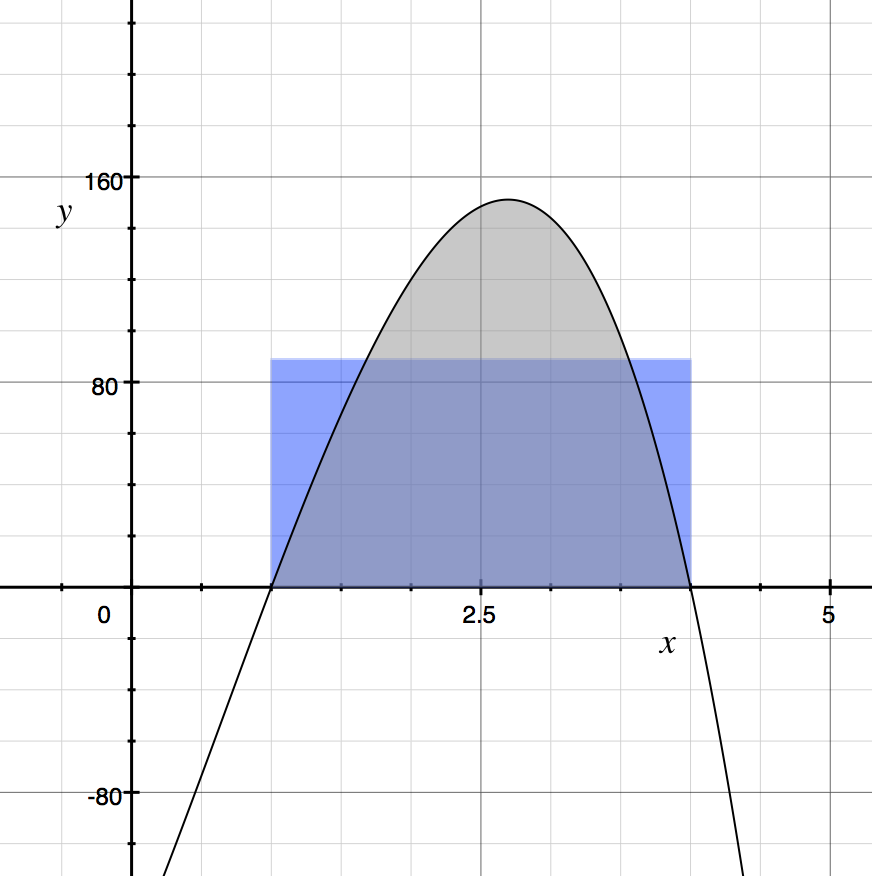
\includegraphics[scale=0.5]{\chapdir/pics/averageintegral}\index{integral!to the average}
\caption[Integrals and Averages]{A rectangle with height at the function's average value has the same area as the integral over the same width.}
\end{centering}
\end{figure}

How can this be?  Imagine if we cut the region up into finitely many pieces.  The average height
is equal to the sum of the heights at every point in our sample group, divided by the number of
samples, $n$, that we have cut the width up into.  
In this case, let us write this sum using the integral sign.

$$
\cfrac{\text{The sum of the heights of} f(x) \text{every} \frac{4-1}{n}}{\frac{4-1}{n}}
$$

But we really ought to use the integral sign, because we don't actually want to cut up the region into
a finite number ($n$) of slices, but an infinite number, with each step being no more than $dx$ wide.
This means we should've written

$$
\cfrac{\int_1^4 f(x)}{\frac{4-1}{dx}} = \frac{\int_1^4 f(x)dx}{4-1}
$$

Because dividing twice is the same as multiplying, our infinitely many additions in the numerator
has suddenly because an infinite number of areas, with infinitely many rectangles being brought
together and summed up --- integrated, each one the height of the function times the infinitely
narrow width $dx$.  In other words, the definite integral over a region, divided by the width of
the region equals the average height of the region.

$$
\frac{\int_a^b f(x)}{b-a} = \frac{F(b)-F(a)}{b-a} = \text{average height}
$$

This is also known as the Fundamental Theorem of Calculus.\index{Fundamental Theorem of Calculus}